\documentclass{article}

\setlength{\evensidemargin}{0in} \setlength{\oddsidemargin}{0in}
\setlength{\textwidth}{6.7in} \setlength{\topmargin}{-1.1in}
\setlength{\textheight}{10.5in}

\usepackage{amssymb, amsthm, amstext, amsxtra, amsmath, amsfonts, amscd }
\usepackage{graphicx, epsfig}
\usepackage{comment, color, cleveref, listings, wrapfig}

\definecolor{dkgreen}{rgb}{0,0.6,0}
\definecolor{gray}{rgb}{0.5,0.5,0.5}
\definecolor{mauve}{rgb}{0.58,0,0.82}
\definecolor{backcolour}{rgb}{0.95,0.95,0.92}

\lstdefinestyle{mystyle}{ frame=tb, backgroundcolor=\color{backcolour}, 
language=R, aboveskip=3mm, belowskip=3mm, showstringspaces=false,
columns=flexible, numbers=none, keywordstyle=\color{blue}, tabsize=3,
numberstyle=\tiny\color{gray}, commentstyle=\color{dkgreen},
stringstyle=\color{mauve}, breaklines=true, breakatwhitespace=true}
\lstset{style=mystyle}

\def\E{\mathbb{E}}
\def\pr{\mathbb{P}}

\renewcommand\baselinestretch{1.2}

\DeclareMathOperator{\sign}{sign}
\DeclareMathOperator{\supp}{supp}

\DeclareMathOperator{\Cov}{Cov}
\DeclareMathOperator{\Var}{Var}
\DeclareMathOperator{\corr}{corr}

\author{Salvador Garcia, s1655274}
\date{10 February 2016}
\title{Assgn3: Students' goals}
  
\begin{document}
\maketitle
\section{Description of the problem} 
  
229 students aged 7-13 from 9 schools were asked whether popularity or sporting ability was most important to them. The aim is to create an appropriate model that takes into account variability between the schools (if necessary).
\textbf{Statistical analysis.}
Introduce the following random variables. Consider the ith student, $i = 1, 2, ... ,N = 229$, and set $Zi = 1$ if popularity is more important to the student than sporting ability, and $Zi = 0$ otherwise.

\section{Likelihood}

\textbf{For this project, openbugs was used}
$Z_i | \theta_k \sim Bern(\theta_k)$, where k is the number of the school the ith student is from, independently given $\theta_k$, $\theta_k \in (0, 1)$.
  
\subsection{Prior case 1: $\theta_1 = \theta_2 = ... = \theta_9$}
In this case, each parameter corresponding to the 9 schools are assumed identical, lets call this parameter $\theta$ and its non-informative prior distribution follows a $beta(1,1)$. The MCMC was run with two chains, the first with initial point $0.1$ and the second $0.9$. As the autocorrelation graph shows, it is not necessary to change the thin parameter. Also, the chain converges relatively fast (Just 501 iterations were used as burning). Finally, the Gelman-Rubin gives us a good conclusion about the convergence. 
  
  \begin{figure}[ht!]
  \centering
  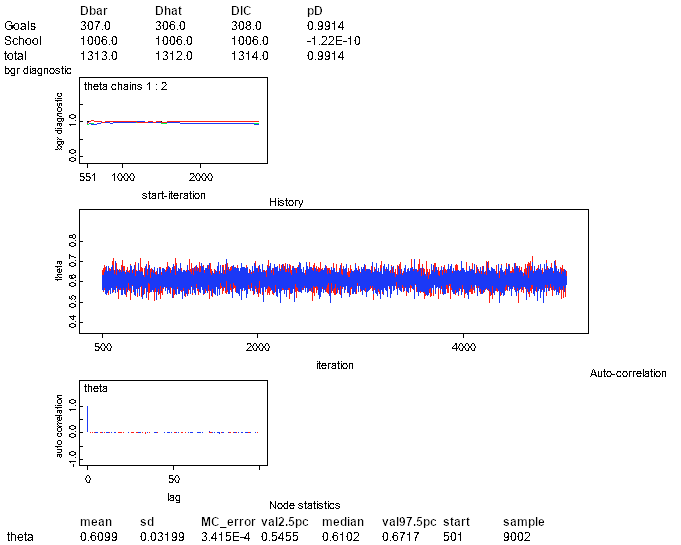
\includegraphics[width=.75\textwidth]{imgs/M1.png}
  \caption{DIC, BGR diagnosis, history and autocorrelation of $\theta$}
  \label{fig:fig1}
  \end{figure}

\newpage
\subsection{Prior case 2: with independent non-informative priors}
Now, we have 9 parameters $(\theta_1, \theta_2, ..., \theta_9)$, each one corresponding to different schools. The prior of each one of these parameters is assumed to be distributed $beta(1,1)$ (non-informative). The MCMC was run with two chains, the first with initial value $\theta_i = 0.1$ for all $i$ and the second $\theta_i = 0.9$ for all $i$. As the autocorrelation graph shows, it was not necessary to change the thin parameter. Again, the chain converge relatively fast (just 1001 iterations were used as burning). Finally, the Gelman-Rubin gives a good conclusion about the convergence of the chains (although for $\theta_2$ there is a very small gap.)

  \begin{figure}[ht!]
  \centering
  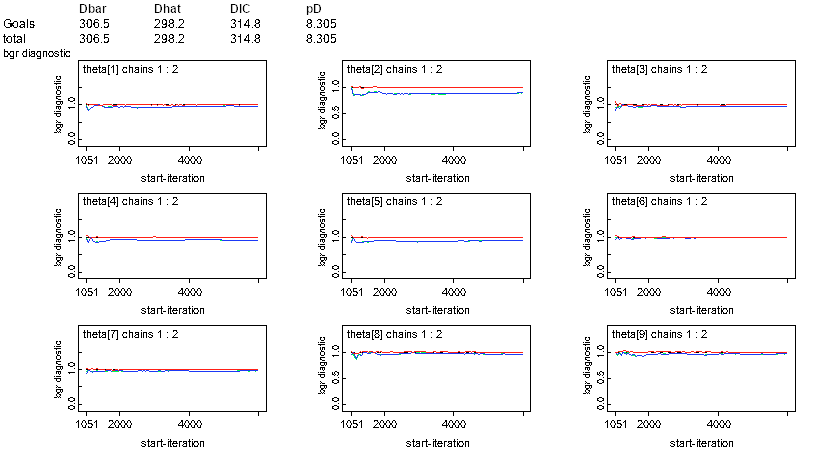
\includegraphics[width=.8\textwidth]{imgs/M2_1.png}
  \caption{DIC and BGR diagnosis for each $\theta_i$, $a$ and $b$. }
  \label{fig:fig2}
  \end{figure}
  
  \begin{figure}[ht!]
  \centering
  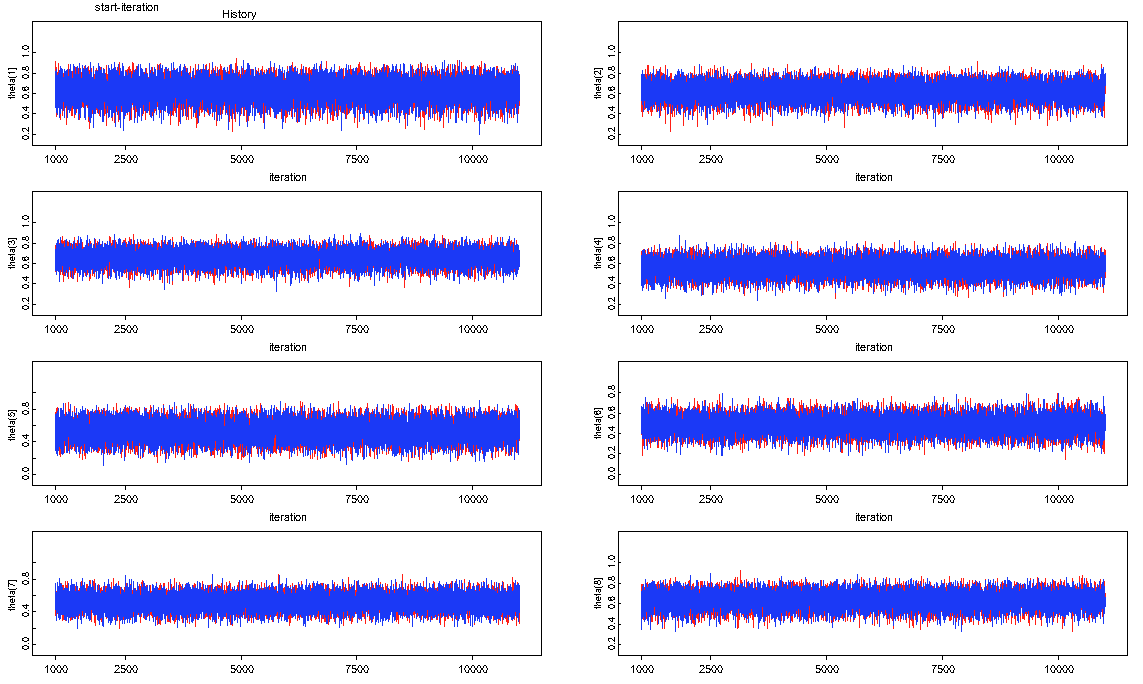
\includegraphics[width=.8\textwidth]{imgs/M2_2.png}
  \caption{History for each $\theta_i$, $a$ and $b$.}
  \label{fig:fig3}
  \end{figure}
  \begin{figure}[ht!]
  \centering
  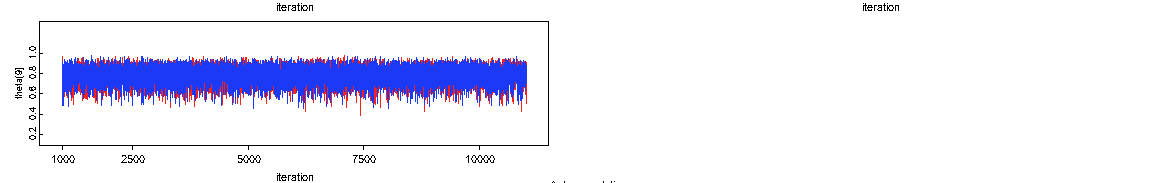
\includegraphics[width=.8\textwidth]{imgs/M2_3.png}
  \caption{History for each $\theta_i$, $a$ and $b$. }
  \label{fig:fig4}
  \end{figure}
  
  \newpage
  \begin{figure}[ht!]
  \centering
  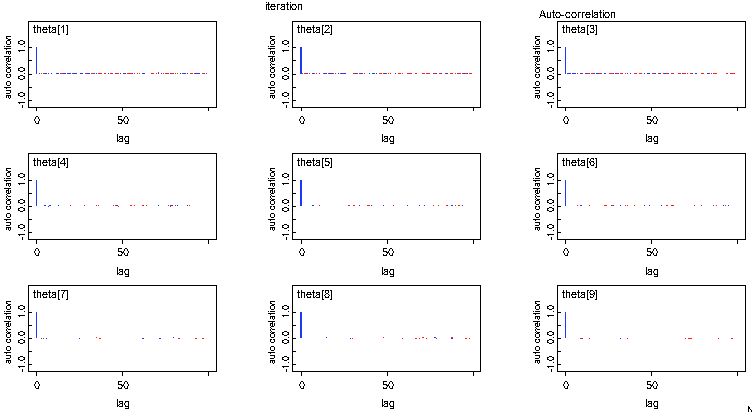
\includegraphics[width=.65\textwidth]{imgs/M2_4.png}
  \caption{Autocorrelation for each $\theta_i$, $a$ and $b$.}
  \label{fig:fig5}
  \end{figure}
  
  \begin{figure}[ht!]
  \centering
  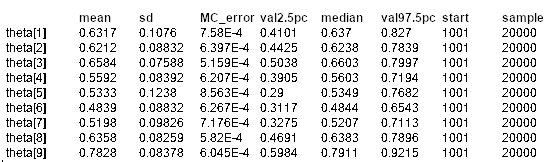
\includegraphics[width=.8\textwidth]{imgs/M2_5.png}
  \caption{Statistics for each $\theta_i$, $a$ and $b$.}
  \label{fig:fig6}
  \end{figure}
   
\subsection{Prior case 3: with a hierarchical exchangeable priors}

In the last example, two different prior distributions will be tested. The first will consider that $a \sim gamma(0.01, 0.01)$ and $b \sim gamma(0.01, 0.01)$ (independently). The second will consider $a \sim |t_3|$ and $b \sim |t_3|$ (independently).

\subsubsection{a,b $\sim gamma(0.01, 0.01)$}
Now, we have 9 parameters $(\theta_1, \theta_2, ..., \theta_9)$ and two additional hyper parameters $a,b$. The prior of each $\theta_i$ is assumed to be distributed $beta(a,b)$ (non-informative) and $a,b$ are assumed to be distributed $gamma(0.01, 0.01)$. The MCMC was run with two chains. For the first chain, the initial values were $a = 10$, $b = 1$, and each $\theta_i = 0.1$ for all $i$. For the second chain, the initial values were $a = 1$, $b = .1$ and each $\theta_i = 0.9$ for all $i$. For this case, the model gives a strong autocorrelation for the parameters $a$ and $b$ (even when thin = 100). Then the prior distribution was changed for a $gamma(0.1, 0.1)$ (same mean, but less variance). Afther this, with a thin = 30 the autocorrelation in $a$ and $b$ was fixed. The chain converges relatively fast (just 501 iterations were used burned). Finally, the Gelman-Rubin gives a good conclusion about the convergence of the chains (although for $a$, $b$ and$\theta_4$ there is a very small gap.)

  \begin{figure}[ht!]
  \centering
  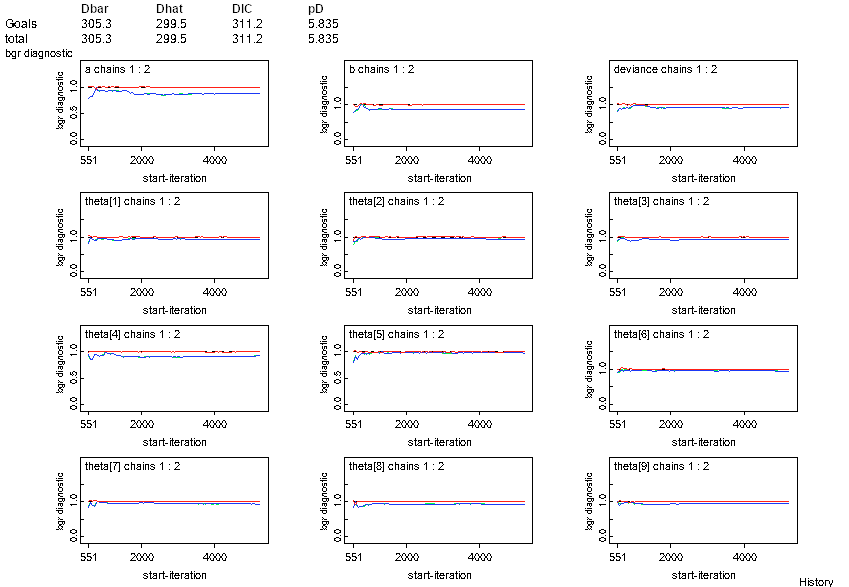
\includegraphics[width=.8\textwidth]{imgs/M3a_1.png}
  \caption{DIC and BGR diagnosis for each $\theta_i$, $a$ and $b$.}
  \label{fig:fig7}
  \end{figure}
  \begin{figure}[ht!]
  \centering
  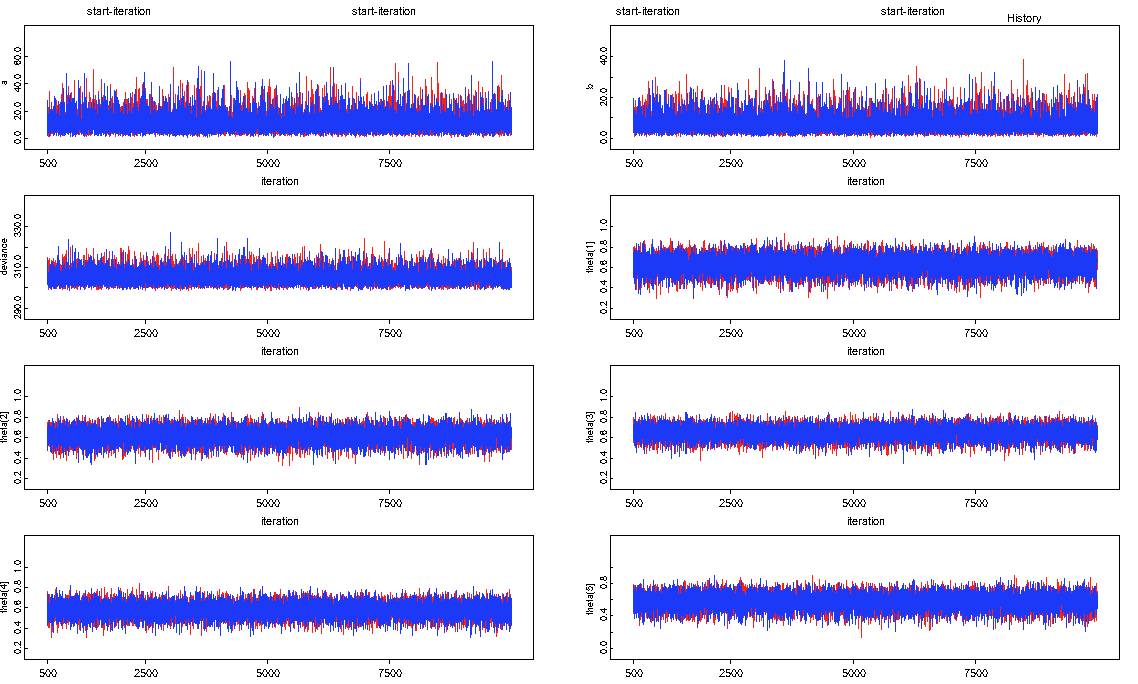
\includegraphics[width=.8\textwidth]{imgs/M3a_2.png}
  \caption{History for each $\theta_i$, $a$ and $b$.}
  \label{fig:fig8}
  \end{figure}
  \begin{figure}[ht!]
  \centering
  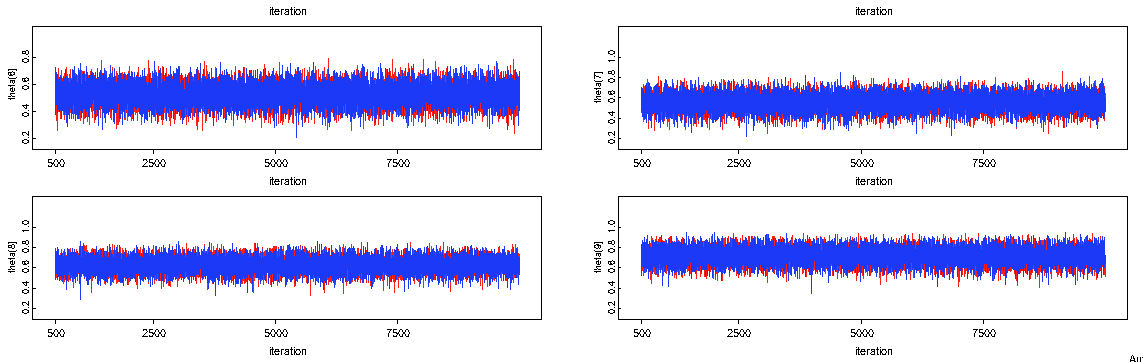
\includegraphics[width=.8\textwidth]{imgs/M3a_3.png}
  \caption{History for each $\theta_i$, $a$ and $b$.}
  \label{fig:fig9}
  \end{figure}
  \begin{figure}[ht!]
  \centering
  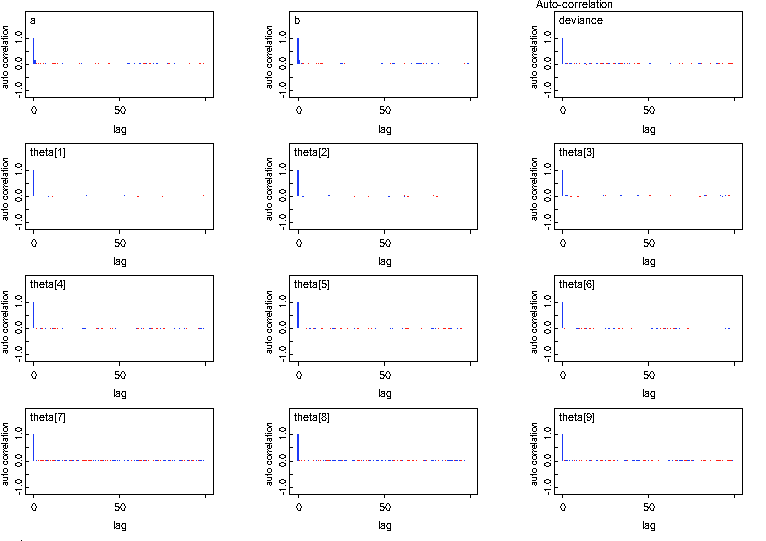
\includegraphics[width=.8\textwidth]{imgs/M3a_4.png}
  \caption{Autocorrelation for each $\theta_i$, $a$ and $b$.}
  \label{fig:fig10}
  \end{figure}
  \begin{figure}[ht!]
  \centering
  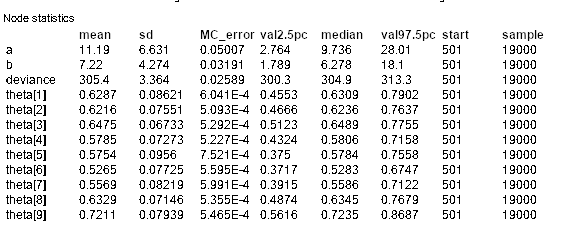
\includegraphics[width=.65\textwidth]{imgs/M3a_5.png}
  \caption{Summary for each $\theta_i$, $a$ and $b$.}
  \label{fig:fig11}
  \end{figure}
  
\newpage
\subsubsection{a,b $\sim |t_3|$}
Again, we have 9 parameters $(\theta_1, \theta_2, ..., \theta_9)$ and two additional hyper parameters $a,b$. The prior of each $\theta_i$ is assumed to be distributed $beta(a,b)$ (non-informative) and $a,b$ are assumed to be distributed $|t_3|$. The MCMC was run with two chains. For the first chain, the initial values were $a = 1$, $b = 10$, and each $\theta_i = 0.1$ for all $i$. For the second chain, the initial values were $a = 10$, $b = 1$ and each $\theta_i = 0.9$ for all $i$.For this experiment, there was a high autocorrelation in the parameters $a$ and $b$, so there was a change the thin parameter (now, equal to 30). The chains converge slow (compared with the other examples, now 4000 iterations were used as burning). Finally, the Gelman-Rubin diagnosis gives us a good conclusion about the convergence of the chains of $\theta_i$, but for $a$, $b$ there is a considerable gap.)
  
  \begin{figure}[ht!]
  \centering
  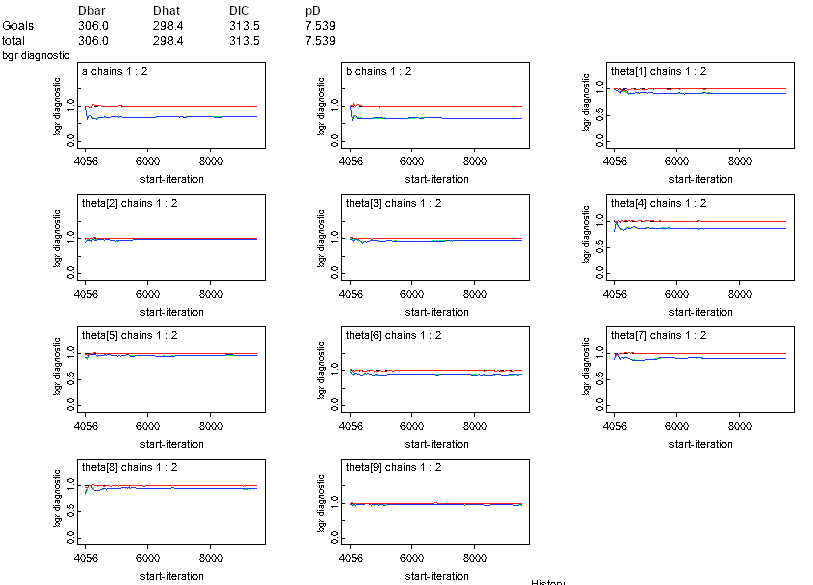
\includegraphics[width=.8\textwidth]{imgs/M3b_1.png}
  \caption{DIC and BGR diagnosis for each $\theta_i$, $a$ and $b$.}
  \label{fig:fig12}
  \end{figure}
  \begin{figure}[ht!]
  \centering
  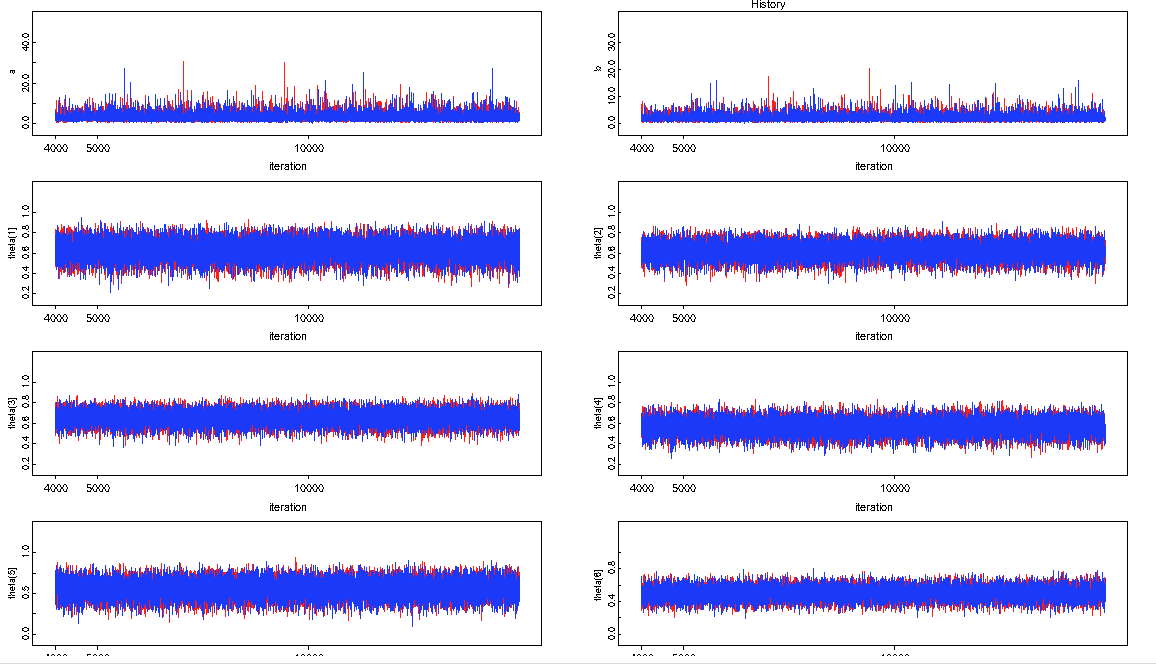
\includegraphics[width=.8\textwidth]{imgs/M3b_2.png}
  \caption{History for each $\theta_i$, $a$ and $b$.}
  \label{fig:fig13}
  \end{figure}
  \begin{figure}[ht!]
  \centering
  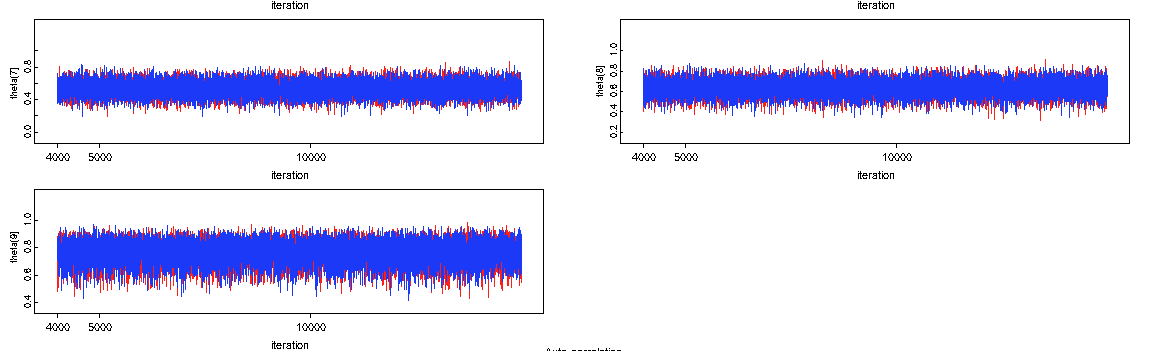
\includegraphics[width=.8\textwidth]{imgs/M3b_3.png}
  \caption{History for each $\theta_i$, $a$ and $b$.}
  \label{fig:fig14}
  \end{figure}
  \begin{figure}[ht!]
  \centering
  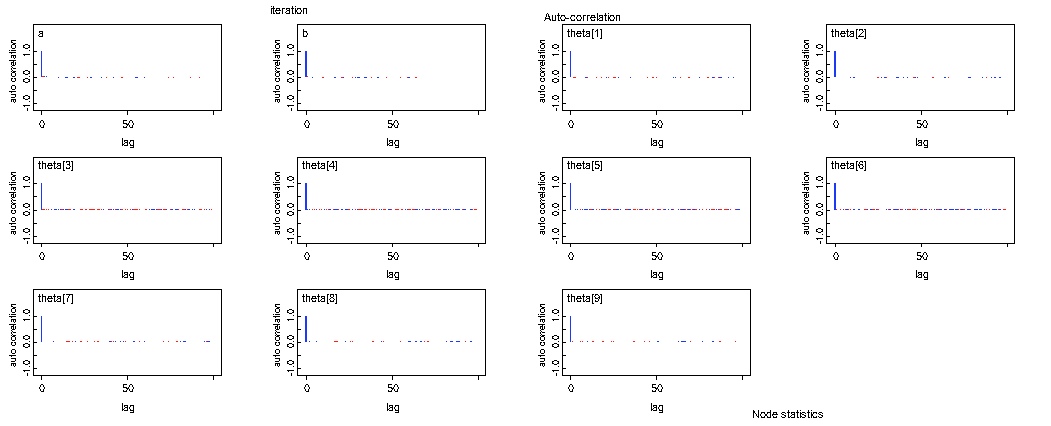
\includegraphics[width=1\textwidth]{imgs/M3b_4.png}
  \caption{Autocorrelation for each $\theta_i$, $a$ and $b$.}
  \label{fig:fig15}
  \end{figure}
  \begin{figure}[ht!]
  \centering
  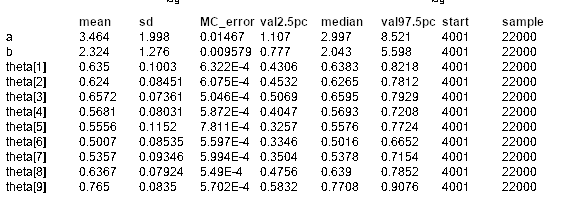
\includegraphics[width=.65\textwidth]{imgs/M3b_5.png}
  \caption{Summary for each $\theta_i$, $a$ and $b$.}
  \label{fig:fig16}
  \end{figure}
\newpage
\section{Conclusions}

For this experiment, the best option was to have a pooled $\theta$. Some experiments that can be done are the following:
\begin{itemize}
\item{Try different priors for the hyper parameters}
\item{Consider another criteria to group the schools}
\end{itemize}

The first point is very important. We can try different prior in order to consider important or not so important the differences between the schools. The second point is an idea to group some schools with the same parameter (for example, the school 1,2,3,4,5 in one group and the school 6,7,8,9 in another). This grouping can be done geographically or with other relevant information. This way, we can reduce the $p_D$ factor of the DIC.

Is important to remark that it is necessary to consider all the values written in the tables of DIC of each model. This way, if we only are worried about fitting, we shoud consider the value \textit{Dhat}. Then, under this assumption, we should select another model as the best one. But as seen in class, we should penalize the number of parameters (this is because of the overfitting, we can have a better $Dhat$, but in prediction this model will have a worse predictions). Again, in the DIC table we can see the value $p_D$ that, according with the theory, is an approximation of the number of parameters. ($p_D \approx p$ with $p$ the number of parameters). In fact, this number is used as a penalization parameter for the DIC (DIC = Dhat + 2pD). 

\begin{table}[ht!] 
\centering
\caption{My caption}
\label{my-label}
\begin{tabular}{l|l|l}
Case                                            & DIC   & pD\\ \hline
$\theta_i$ are equal with non informative prior (pooled) & 308.0 & 0.9914\\
Independent non informative priors              & 314.8 & 8.305 \\
Hierarchical exchangeable prior (Gamma)         & 311.2 & 5.835\\
Hierarchical exchangeable prior ($|t_3|$)       & 313.5 & 7.538
\end{tabular}
\end{table}

Now, interpreting the results according to the problem, when we select the first model ($\theta_i$ are equal with non informative prior (pooled)), we arrive at a conclussion that $\theta = .6099$, i.e. that 60\% of the students will prefer popularity over sporting ability. This can be given with the credibility interval of $(0.5455, 0.6717)$.

Another point is that, in the models of exchangeable prior, the sd deviation of each $\theta_i$ is less than the second model (Independence). Also, the mean of $\theta_i$ in the the hierarchical model is closer to the mean of $\theta$ the first model (partially pooling in direction to a common mean). 
This is directly related with the assumption that in the hierarchical models the have a dependency between them. 
\end{document}
  